  \begin{figure*}[ht]
      \centering
      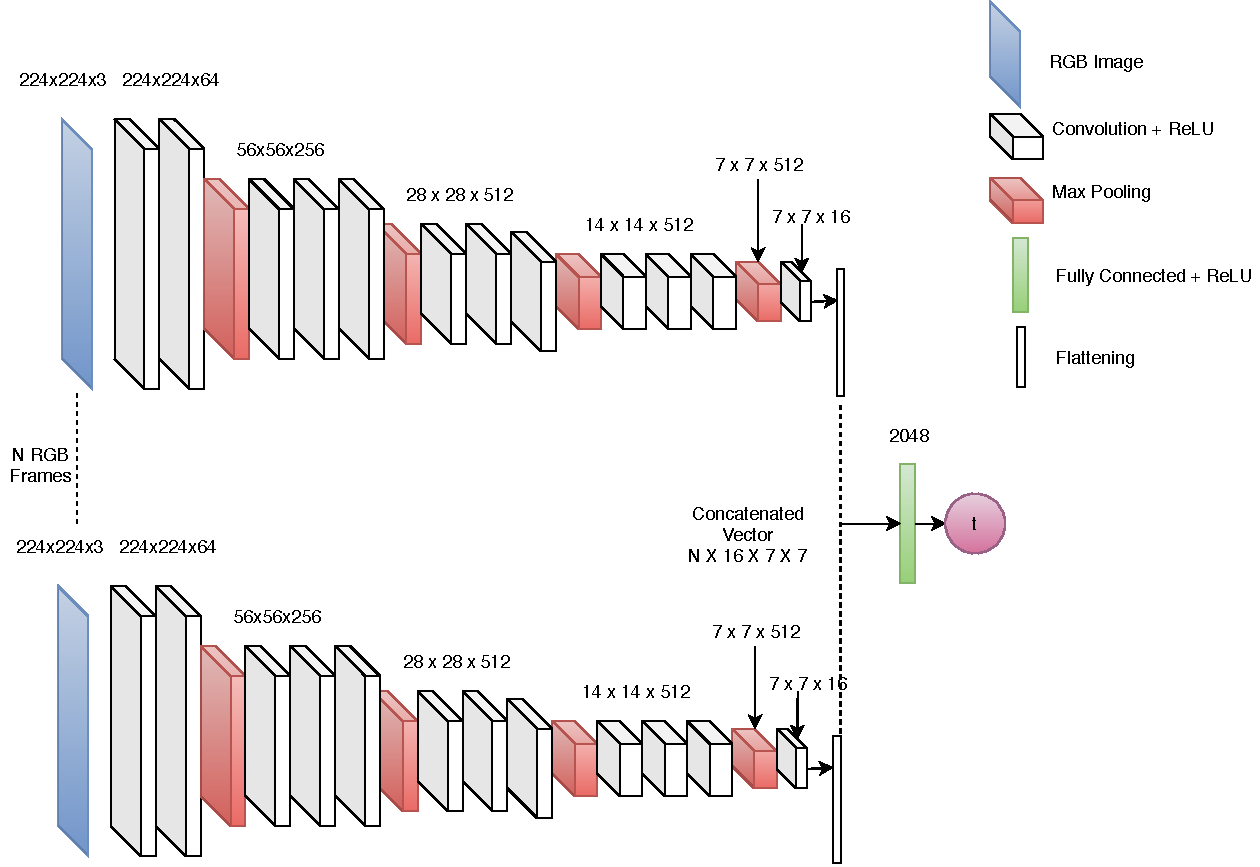
\includegraphics[height=7.0cm, width=12cm]{figs/vgg_2.pdf}
      \caption{Our model with VGG-16 as backbone where the final output is time to collision denoted as $t$ }
      \label{fig:model}
  \end{figure*}

Our goal is to predict the time at which at least one person is going to come within a meter distance of the mobile setup using only a monocular image sequence of $N$ frames. The video is recorded at $10$ fps and thus a sequence of $N$ frames, including the current frame and past $(N-1)$ frames, correspond to the history of $\frac{N-1}{10}$ seconds. We first provide a formal definition of the task and then the details of network architecture for reproducibility.   

\section{Problem Formulation - Classification or Regression?}
Learning time to near-collision can be formulated as a multi-class classification into one of the 60 classes where $i^{th}$ class corresponds to time range between $(\frac{i-1}{10}, \frac{i}{10}]$ seconds. The disadvantage of training it as a classification task is that all the mispredictions are penalized equally. For example, let us consider two different mispredictions given the same ground truth of 0.5 seconds - one where the network categorized it into the class $(0.6, 0.7]$ and other when the network predicted $(5.5, 5.6]$. The multi-class cross-entropy loss on both of these will be equal while we want the latter to be penalized much more than the former. One of the solutions is to design a differentiable loss function which keeps this preference in mind. Another solution is to formulate it as a regression problem and use the mean-squared error as the loss function. In this paper, we formulated it as a regression problem as follows:
$$
%t = f(image_{1}, image_{2}, \hdots, image_{N}) \text{ where } t \in [0, 6]
t = f(I_{1}, I_{2}, \hdots, I_{N}) \text{ where } t \in [0,6]
$$

\section{Network Architecture}
%% Why I chose VGG-16?
%% ImageNet do not have a person class, thus the network was fine-tuned on PASCAL VOC dataset 
%% We propose a N-stream network where each stream takes in the $i^{th}$ image  
VGG-16 \cite{vgg} is a 16-layer convolutional neural network which won the localization task in ImageNet Challenge 2014. It used parameter efficient $3 \times 3$ convolutional kernels pushing the depth to 16 weight layers. It was shown that its representations generalize well to other datasets achieving state-of-the-art results. We propose a multi-stream VGG architecture as shown in Fig. \ref{fig:model} where each stream takes a $224 \times 224$ RGB frame as input to extract spatial features . These spatial features are then concatenated across all frames preserving the temporal order and then fed into a perceptron to output time to collision. \\

% The inputs to the network are short N-frame clips corresponding to a temporal footprint of $\frac{N-1}{10}$ seconds. The concatenated features are fed into a 2 layer perceptron to give a single real-valued output. The network is trained using mean squared error as loss on the output. \\

\textbf{Feature Extraction from VGG-16} We extracted the features of dimensions  7$\times$7$\times$512 from the last max pool layer of VGG-16. These features pass through an additional convolution layer to reduce the feature size to 7$\times$7$\times$16 and then flattened. These flattened features for each frame are concatenated into a vector and fed into the successive fully-connected layer of size 2048 which finally leads to a single neuron denoted as $t$ in Fig. \ref{fig:model}.  
%The network is trained using mean squared error as loss on the output.    \\
%% Which layer of VGG-16; I also added a conv layer from 512 channels to 16. 

In this network, the convolutional operators used spatial 2D kernels. A major question in current video architectures is whether these 2D kernels should be replaced by 3D spatio-temporal kernels \cite{i3d}. To answer this we also experimented with 3D spatio-temporal kernels and report the results in following section. \\

\textbf{Training N-stream VGG} We initialized the VGG-16 network using ImageNet-pretrained weights. As the ImageNet dataset does not have a person class, we fine-tuned the network weights on PASCAL VOC \cite{pascalVOC} dataset. Using these weights as initialization, we train a multi-stream architecture with shared weights. The network is trained using the following loss function.
$$
L_{MSE} = \frac{1}{2}||t_{true} - f(I_1, I_2, \hdots, I_N)||^{2}
$$
Here, $L$ is the mean squared loss between the predicted time, \emph{i.e.}, $f(I_1, I_2, \hdots, I_N)$ and ground truth time denoted as $t_{true}$. \\
The loss is optimized using mini-batch gradient descent of batch size 24 with the learning rate of $0.001$. The training data is further doubled by applying horizontal flip transformation.
%% Leaning rate, gradient descent, batch size